\documentclass{article}
\usepackage[margin=1.5cm]{geometry}
\usepackage{microtype} % Slightly better kerning
\usepackage{graphicx}
\graphicspath{ {./figs/} }
\usepackage[colorlinks=true]{hyperref}
\setlength{\parindent}{0pt}
\setlength{\parskip}{1em}
\usepackage{fancyhdr} % Needed to adjust page numbering
\usepackage{lastpage} % Counts total number of pages

\pagestyle{fancy}
\fancyhf{}
\renewcommand{\headrulewidth}{0pt} % Remove header line
\cfoot{\thepage \hspace{1pt} of \pageref*{LastPage}} % Customize page nums

\usepackage{amsmath}
\usepackage{upgreek}

\usepackage{array} % New env. for equation conditions where aligned
\newenvironment{conditions}[1][where:] 
  {#1 \begin{tabular}[t]{>{$}l<{$} @{${}={}$} l}}
  {\end{tabular}\\[\belowdisplayskip]}

\usepackage{listings}

\title{Spatial Interpolation Notes}

\begin{document}
\maketitle

\section{Introduction}

We want to use interpolation because it is reasonable to assume that spatially distributed variables are also spatially correlated.
It is not always true, but often worth exploring as part of an analysis.
There are multiple different methods to interpolate data that depend on different underlying assumptions.
These methods are described below.

\begin{center}
    \fbox{Information from \href{https://desktop.arcgis.com/en/arcmap/10.3/tools/3d-analyst-toolbox/how-kriging-works.htm}{ARCGIS} and Applied Spatial Data Analysis With R (2013) unless listed otherwise}
\end{center}

There are two main methods used to interpolate data and estimate a surface for geospatial data:

\begin{itemize}
    \item Inverse distance weighting (IDW) and spline methods
    \item Kriging
\end{itemize}

IDW and splines are deterministic interpolation methods as they are directly based on the surrounding values or smoothed formulas.
Kriging is different as it uses autocorrelation and takes position into account in the statistical models.
Kriging uses a certain number of neighbouring points, or all points within a specified radius (cf kNN).

The general formula for IDW and kriging is:

\[\hat{Z}(s_{0} )=\sum_{i=1}^{N} w(s_{i}) Z (s_{i})\]

\begin{conditions}
Z(s_{i}) & the measured value at the $i$th location \\
w(s_{i}) & an unknown weight for the measured value at the $i$th location \\
s_{0} & the prediction location \\
N & the number of measured values
\end{conditions}

The difference between IDW and kriging is that in IDW, $w(s_{i})$ only depends on distance to prediction location.
In kriging $w(s_{i})$ also depends on autocorrelation i.e. spatial relationship between prediction locations.

\section{Inverse distance weighting (IDW)}

IDW determines cell values using a linearly weighted combination of surrounding values.
The weights are function of the inverse distance.
The general form for the IDW function is:

\[\hat{Z}(s_{0})= \frac{\sum_{i=1}^{n} w(s_{i}) Z(s_{i})}{\sum_{i=1}^{n} w (s_{i})}\]

\begin{conditions}
    Z(s_{i}) & the measured value at the $i$th location \\
    w(s_{i}) & $||s_{i} - s_{0}||^{-p}$ \\
    || \cdot || & Euclidean distance \\
    p & an inverse distance weighting power, defaulting to 2
\end{conditions}

The value of $p$ determines how much closer values are preferred.
As $p$ increases, IDW approaches a one-nearest-neighbour interpolation model.
$p$ can be selected using cross-validation.

Another way to control IDW interpolation is through selecting the number of neighbouring observations to include.
This can improve speed of interpolation, and may be used when there is reason to believe that distant points have little correlation.
There are two approaches for varying the number of points used for interpolation:

\begin{enumerate}
    \item Varying search radius 
    \begin{itemize}
        \item The number of points to include is fixed, and the radius changes to include that set number
        \item Depends on the density of observations fluctuating
        \item The maximum radius can also be set, in which case all points will be included if that max radius is reached before $n$
    \end{itemize}
    \item Fixed search radius
    \begin{itemize}
        \item Set a radius and minimum number of points
        \item If $n <$ minimum number of points at set radius, the radius increases until the minimum is reached.
    \end{itemize}
\end{enumerate}

In addition to these two approaches, barriers can be created to limit the searches for neighbouring points, i.e. only search for this side of a river.

\section{Kriging}

One of the key benefits of kriging is that in addition to using autocorrelation, it is able to estimate uncertainty in the interpolation.
It can do this because it is based on a spatial arrangement of empirical observations, rather than a presumed model of spatial distribution.
Although kriging preferentially weights closer observations, its use of autocorrelation means that clusters are not over-fit i.e. lowering bias as each point in a cluster provides less information than a single point.

The kriging predictor is an "optimal linear predictor" and an exact interpolator.
This means that prediction error is each interpolated value is calculated to minimize the prediction error for that point.
It also means that the interpolated value for sampled points is equal to the actual value, and all interpolated values will be the Best Linear Unbiased Predictors (BLUPs).

Kriging is only helpful where there is at least moderate spatial autocorrelation.
If there is not, then simpler methods like IDW, will generally perform as well as kriging.

\subsection{Assumptions in kriging}

\begin{center}
    \fbox{Information for assumptions from \href{https://www.publichealth.columbia.edu/research/population-health-methods/kriging-interpolation}{Columbia}}    
\end{center}

For kriging to be used, there are a number of assumptions/conditions to be met.
These conditions can be checked in exploratory data analysis.

\begin{enumerate}
    \item Assumption of intrinsic stationarity
    \begin{itemize}
        \item Means that the joint probability distribution does not vary across the study space, so the same parameters (e.g. mean, range and sill etc) are valid across the space
        \item Means one variogram is valid across the space
    \end{itemize}
    \item Assumption of isotropy
    \begin{itemize}
        \item Uniformity in all directions (semivariance identical in all directions)
    \end{itemize}
\end{enumerate}

By making these assumptions, we are assuming that the samples are randomly generated by the function $Z(s)$ with a mean ($m$) and residual ($e(s)$).

\[Z(s) = m + e(s)\]

\begin{conditions}
    E\left(Z(s)\right) & $m$
\end{conditions}

The assumption of \textit{intrinsic stationarity} and \textit{isotropy} can be relaxed to create models where the mean varies spatially.
In instances like this, the measured values can be assumed to be randomly generated by a linear function of known predictors $X_j(s)$.

\begin{equation}
    \begin{split}
        Z(s) & = \sum_{j=0}^p X_j(s)\beta_j + e(s) \\
        & = X\beta + e(s)
    \end{split}    
\end{equation}


\subsection{Creating a prediction map with kriging}

There are two steps:

\begin{enumerate}
    \item Create the variograms and covariance functions to estimate the spatial autocorrelation values that depend on the model of autocorrelation (fitting a model).
    \item Predict the unknown values
\end{enumerate}

\subsubsection{Variography (spatial modelling/structural analysis)}

There are often too many pairs of spatial points to calculate and plot the distance for each pair.
Instead, spatial distances are put into lag bins i.e. all points in the range $40m < h \le 50m$ of point A, and calculate the semivariance.
The semivariance is equal to half the variance of the differences between all possible points spaced a constant distance apart.
Assuming \textit{isotropy} and \textit{intrinsic stationarity}, we can generalise the distances between points and use the distance $||h||$ rather than the vector $\textbf{h}$, i.e. use bins.

\[\hat{\gamma} (\tilde{h}_j) = \frac{1}{2N_h}\sum_{i=1}^{N_h}\left(Z(s_i) - Z(s_i + h)\right)^2, \text{ } \forall h \in \tilde{h}_j\]

\begin{conditions}
    Z(s_{i}) & the measured value at the $i$th location \\
    \hat{\gamma} (\tilde{h}_j) & sample variogram \\
    N_h & sample data points \\
    \tilde{h}_j & distance bins (intervals)
\end{conditions}

Plotting the distance vs semivariance produces an empirical semivariogram.
Closer items should be more similar, therefore lower semivariance.
The opposite is true for further points.

A model is fit to the empirical semivariogram (cf regression).
Different types of models can be fit the the semivariogram, and the optimal model can be selected using metrics like RMSE, MLE, and Bayesian methods:

\begin{itemize}
    \item Spherical (most common)
    \item Circular
    \item Exponential
    \item Gaussian
    \item Linear
\end{itemize}

\begin{figure}[h]
    \centering
    \label{Kriging variogram model shapes}
    \caption{Different types of models used in spatial modelling \href{https://www.publichealth.columbia.edu/research/population-health-methods/kriging-interpolation}{(Poilou 2008)}. a) Linear semi-variogram; (b) spherical semi-variogram; (c) exponential semi-variogram; and (d) power semi-variogram}
    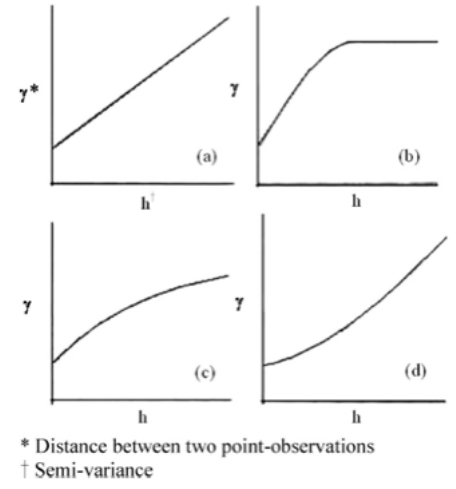
\includegraphics[width=10cm]{semivariogram-models.png}
\end{figure} 

There are a number of key points on the figures:

\begin{itemize}
    \item Range
    \begin{itemize}
        \item The Range is the point at which the semivariance first levels off
        \item Items within the range are autocorrelated (distance matters)
        \item Items outside the range are not autocorrelated (distance no longer changes the semivariance)
    \end{itemize}
    \item Sill 
    \begin{itemize}
        \item The Sill is the height at which the semivariance levels off to
    \end{itemize}
    \item Nugget
    \begin{itemize}
        \item The minimum value of semivariance ($\gamma (h = 0)$)
        \item Theoretically there is no semivariance when $h=0$, but in reality it is present due to measurement error or spatial sources of variation at distances smaller than the sample interval (or both)
    \end{itemize}
    \item Partial Sill
    \begin{itemize}
        \item Amount of semivariance between Sill and the Nugget
    \end{itemize}
\end{itemize}

\subsubsection{Predictions}

Now a model has been fit to the semivariance and autocorrelation can be observed, predictions can be made within the domain.
Kriging differs from IDW as it uses the semivariogram to calculate the weights.
There are a number of methods used in kriging:

\begin{enumerate}
    \item Ordinary kriging
    \begin{itemize}
        \item Assumes the constant mean is unknown
    \end{itemize}
    \item Universal kriging
    \begin{itemize}
        \item Assumes there's a prevailing trend, relaxing the assumption of stationarity for the mean, but maintaining a constant variance
        \item Trend is modelled with polynomial function, and subtracted from observed
        \item Semivariogram is modelled on the residuals to produce autocorrelations
    \end{itemize}
    \item Block kriging
    \begin{itemize}
        \item Estimates averaged values over gridded “blocks” rather than single points
        \item These blocks often have smaller prediction errors than are seen for individual points
    \end{itemize}
    \item Covariate kriging
    \begin{itemize}
        \item Additional observed variables (which are often correlated with each other and the variable of interest) are used to enhance the precision of the interpolation of the variable of interest at each location
    \end{itemize}
    \item Poisson kriging
    \begin{itemize}
        \item Used for incidence counts and disease rates 
    \end{itemize}
\end{enumerate}

\subsection{Limitations}

\begin{center}
    \fbox{Information for limitations from \href{https://www.publichealth.columbia.edu/research/population-health-methods/kriging-interpolation}{Columbia}}    
\end{center}

There are a number of limitations of kriging.

\begin{enumerate}
    \item Since the weights of the kriging interpolator depend on the modeled variogram, kriging is quite sensitive to mis-specification of the variogram model
    \item Similarly, the assumptions of the kriging model (e.g. that of second-order stationarity) may be difficult to meet in the context of many environmental exposures
    \begin{itemize}
        \item Some newer methods (e.g. Bayesian approaches) have thus been developed to try and surmount these obstacles
    \end{itemize}
    \item In general, the accuracy of interpolation by kriging will be limited if the number of sampled observations is small, the data is limited in spatial scope, or the data are in fact not amply spatially correlated
    \begin{itemize}
        \item In these cases, a sample variogram is hard to generate, and methods such as land-use regression may prove preferable to kriging for spatial prediction
    \end{itemize}
\end{enumerate}



\section{Natural Neighbour}

Natural neighbour is a local method that examines samples near the point of interest and evaluates the relative overlap with their areas.
The relative overlaps are then used to create the weights for interpolation.
Because of this, it is also known as "area-stealing" (Sibson) interpolation.
Natural neighbour interpolation therefore does not infer trends that are not already present in the data, and the surface passes through the points, and is smooth in between.

The areas are called Voronoi (Thiessen) polygons.
Voronoi polygons are created by examining the space around points and drawing the boundary so that every place inside the boundary is closest to the polygon's point than any other.
Formally this is written as:

\[R_{k} = \left\{x \in X \mid d(x, P_{k}) < d(x, P_{j}),  \text{ } \forall j \neq k)\right\}\]

\begin{conditions}
    R_{k} & Voronoi polygon of point $k$ \\
    P_{k} & Point $k$ \\ 
    P_{j} & Neighbouring point $j$
\end{conditions}

An example of this can be seen in the figure below.

\begin{figure}[h]
    \centering
    \caption{Natural neighbour method of interpolation}
    \label{Natural neighbour method of interpolation}
    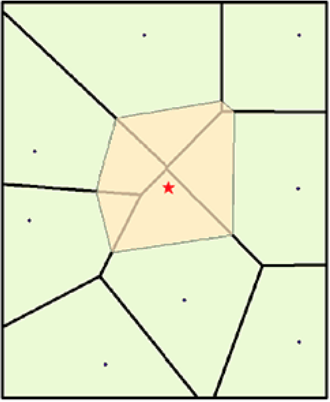
\includegraphics[width=5cm]{natural-neighbour.png}
\end{figure}

\section{Splines}

Splines are a smoothing function that pass through all the input points and attempt to create a smooth surface between them.
As such, it is best for gently varying surfaces e.g. pollution concentrations.
The surface is fit to a specified number of neighbouring input points.
The basic spline is also known as a thin plate interpolation.
There are two conditions that minimum curvature splines must follow:

\begin{enumerate}
    \item The surface must pass through all data points
    \item The surface must have minimum curvature i.e. minimize the cumulative sum of squares of the second derivative terms of the surface at each point
\end{enumerate}

One possible issue with thin plate interpolation is that there may be rapid change in first derivatives around each data point.
Increasing the number of points used for interpolation can help to smooth the surface as the cell is influenced by a greater number of more distant points.
Splines create rectangular regions of equal size, with the same number in the $x-$ and $y-$ directions.
Each region must contain at least 8 points, but different densities resulting from data that is not uniformly distributed can lead to regions containing different numbers of points.

Generally, the spline formula is:

\[S(x, y) = T(x, y) + \sum_{j=1}^{N} \lambda_{j} R(r_{j})\]

\begin{conditions}
    N & total number of points to be used in interpolation \\
    \lambda_{j} & coefficients found by the solution of a system of linear equations \\
    r_{j} & the distance from the point $(x,y)$ to the $j$th point
\end{conditions}

There are two spline types, which define the terms $T(x, y)$ and $R(r_{j})$ differently.

\subsection{Regularized splines}

A regularized spline creates a smooth and gradually changing surface, allowing values outside those observed in the data.

\[T(x, y) = a_{1} + a_{2}x + a_{3}y\]

\begin{conditions}
    a_{i} & coefficients found by the solutions of a system of linear equations
\end{conditions}

and, 

\[R(r) = \frac{1}{2 \pi} \left\{\frac{r^2}{4}\left[\ln \left(\frac{r}{2 \uptau}\right) + c - 1 \right] + \uptau^2\left[K_0 \left(\frac{r}{\uptau}\right) + c + \ln \left(\frac{r}{2 \pi}\right)\right]\right\}\]

\begin{conditions}
    r & the distance between the point and the sample \\
    \uptau^2 & the Weight parameter \\
    K_0 & the modified Bessel function \\
    c & a constant equal to 0.577215
\end{conditions}

In regularized splines, the Weight parameter ($\uptau^2$) specifies the weights attached to the third derivatives terms during minimization.
Larger weights result in smoother surfaces and smooth first-derivative surfaces.
Typical values range between 0 and 0.5.

\subsection{Tension splines}

A tension spline creates a less smooth surface with values more tightly constrained by the sample data range.

\[T(x, y) = a_{1} \]

\begin{conditions}
    a_{1} & a coefficient found by the solutions of a system of linear equations
\end{conditions}

and, 

\[R(r) = - \frac{1}{2 \pi \varphi^2} \left[\ln\left(\frac{r \varphi}{2}\right) + c + K_0 \left(r \varphi\right)\right]\]

\begin{conditions}
    r & the distance between the point and the sample \\
    \varphi^2 & the Weight parameter \\
    K_0 & the modified Bessel function \\
    c & a constant equal to 0.577215
\end{conditions}

The tension method differs from regularized splines as it attaches the Weight parameter ($\varphi^2$) to first-derivative terms, not third-derivative terms.
Larger values of $\varphi^2$  lower the tension and result in a coarser surface as the first-derivative surface is not smooth, passing through all the points.
$\varphi^2 = 0$ results in a basic thin plate surface.
Typical values range between 0 and 10.

\section{Datacamp: Visualizing geospatial data in R}

\begin{itemize}
    \item \textit{ggmap} package very useful for quickly producing static spatial plots
    \begin{itemize}
        \item \textit{ggmap:get\_map(long, lat)} pulls basemap based lat long
        \item \textit{ggmap(*ggmap*, base\_layer = ggplot(df, aes(long, lat))) + geom\_point()} allows you to plot layers over map and retain same aes() e.g. for faceting
    \end{itemize}
    \item Different types of spatial data
    \begin{itemize}
        \item Point data
        \item Line data - assumes points connected by straight lines
        \item Polygon data
        \begin{itemize}
            \item Data associated with enclosed area of points
            \item \textit{ggplot2::geom\_poly()}
        \end{itemize} 
        \item Raster (grid) data
        \begin{itemize}
            \item Regular grid specified by origin and steps in x and y axis, and data is associated with cells in grid
            \item \textit{ggplot2::geom\_tile(aes(fill = *var*))} used to create raster
        \end{itemize}
    \end{itemize}
    \item Polygon data
    \begin{itemize}
        \item Difficult to described
        \begin{itemize}
            \item Order of joining up points matters
            \item Polygons may be broken up e.g. by river therefore needing multiple polygons to describe it
        \end{itemize}
    \end{itemize}
    \item \textit{sp} data structures better that \textit{dataframes} for storing spatial data as don't have to repeat info like groups and order for polygons, and contains information about the coordinate sytem itself, which is useful when working with multiple systems/for sharing
    \item \textit{spdf} is an \textbf{S4} data type
    \begin{itemize}
        \item Useful adaptation of \textit{sp} structure as also contains dataframe
        \item Items are \textbf{slots} that are accessed with the \textit{@} symbol e.g. \textit{spdf@polygon}
        \begin{itemize}
            \item Each \textbf{slot} contains a list that is \textit{another} \textbf{S4} object (e.g. Polygons) (see Fig. \ref{spdf data structure})
            
            \begin{figure}[h]
                \centering
                \caption{\textit{spdf} data structure}
                \label{spdf data structure}
                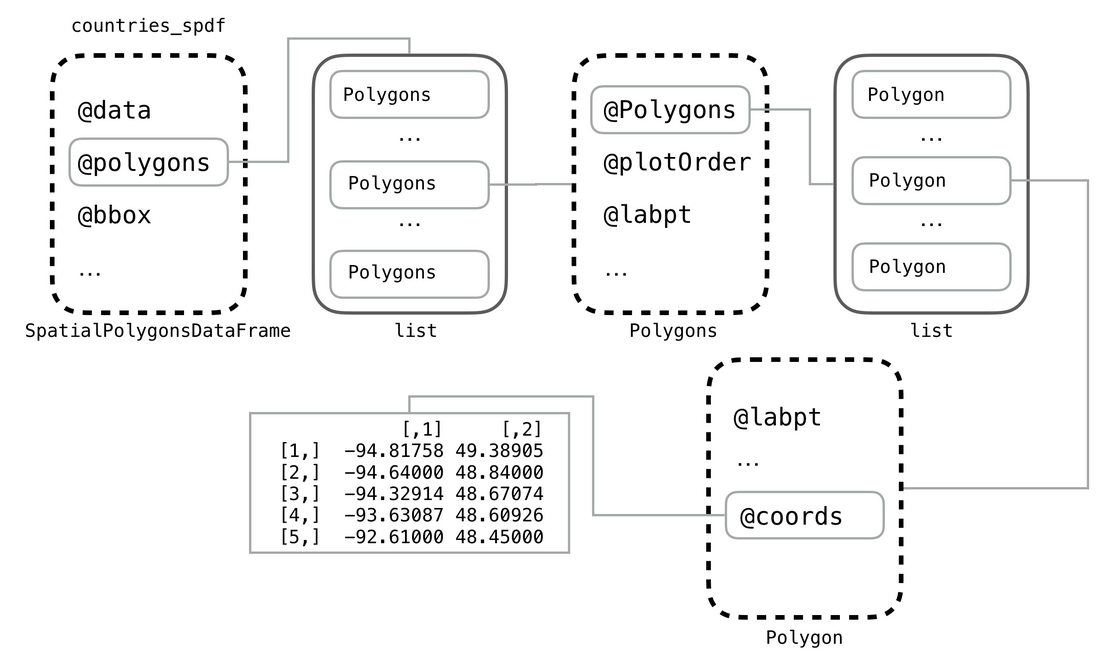
\includegraphics[width=15cm]{spdf.png}
            \end{figure} 

            \item Can pull information as with normal dataframes using $\$$ symbol e.g. 
            \begin{itemize}
                \item \textit{is\_nz = countries\_spdf\$name == ``New Zealand''}
                \item \textit{nz = countries\_spdf[is\_nz, ]}
            \end{itemize}
        \end{itemize}
    \end{itemize}
    \item \textit{tmap} package designed to plot spatial data, rather than requiring dataframe format, like \textit{ggplot2}
    \begin{itemize}
        \item \textit{tm\_shape()} adds basemap
        \item \textit{tm\_raster()} creates choropleth for rasters
        \item \textit{tm\_fill()} creates choropleth for polygons
        \item Can save interactive \textit{leaflet} map using \textit{tmap\_save(filename = *.html)}
    \end{itemize}
    \item \textit{raster} package better to work with raster data than \textit{sp} and \textit{ggplot2}
    \begin{itemize}
        \item Creates an \textbf{S4} object
        \item More efficient as stores data in matrix like format, where each value is associated with a cell in the raster grid
        \begin{itemize}
            \item Multiple matrices act as layers to provide more information
            \begin{itemize}
                \item \textit{Multi-band/multi-layer} rasters
                \item e.g. single band for red/green/blue light to produce colours
            \end{itemize}
            \item Reduces reproducing the same grid
        \end{itemize}
        \item \textit{rasterVis::levelplot()} good for quickly visualizing rasters
    \end{itemize}
    \item \textit{classInt::classIntervals()} useful to bin continuous variables for choropleths
    \item \textit{rgdal::readOGR} used to read in shape files (polygons)
    \item \textit{proj4string()} allows you to define the coordinate reference system (CRS) and projection when no present, or print it where it is present
    \item \textit{rgdal::spTransform()} used to transform CRS
    \begin{itemize}
        \item \textit{tmap} does the transformation automatically
    \end{itemize}
    \item \textit{sp::merge(spdf, df, by.x, by.y)} used to add new information to sp dataframe

    \begin{itemize}
        \item \textit{spdf} have information on \textit{x} number of \textbf{poylgons} (\textit{not observations, like a normal df})
        \item Both \textit{@data} and \textit{@polygon} slots contain an \textit{@ID} slot to match the data to the polygons
        \begin{itemize}
            \item Need to make sure you match them when adding new data otherwise may become unordered
        \end{itemize}
    \end{itemize}
\end{itemize}

\section{Datacamp: Spatial analysis with sf and raster in R}

\begin{itemize}
    \item \textit{sf} package new way to read and use spatial information
    \begin{itemize}
        \item \textit{sf::st\_read(``file.sh'')} reads shape files into dataframe with special \textit{geometry} \textbf{list column}
        \begin{itemize}
            \item Means they can be manipulated like standard dfs, e.g. using \textit{dplyr} etc
        \end{itemize}
        \item Also save \textbf{metadata} that can be seen with \textit{head()} call
    \end{itemize}
    \item \textit{raster}
    \begin{itemize}
        \item \textit{raster::brick(``file.tif'')} reads in single band raster data
        \item \textit{raster::raster(``file.tif'')} reads in single band raster data
    \end{itemize}
    \item \textit{sf::st\_area()} calculates area of individual features
    \begin{itemize}
        \item Produces a vector \textbf{with units} in metadata
        \begin{itemize}
            \item Means you have to use \textit{unclass()} function to remove units for calculations e.g. \textit{df \%$>$\% filter(unclass(areas) $>$ 3000)}
        \end{itemize}
    \end{itemize}
    \item \textit{sf::st\_area()} calculates area of individual features
    \item \textit{sf::st\_length()} calculates length of individual
    \item \textit{raster::plotRGB()} used to plot multi-band raster images quickly (if bands correspond to RGB)
    \begin{itemize}
        \item \textit{plot()} creates plots for each band separately
    \end{itemize}
    \item To \textbf{add} CRS information:
    \begin{itemize}
        \item For \textit{sf} data:
        \begin{itemize}
            \item \textit{sf::st\_crs()} shows you the current CRS information
            \begin{itemize}
                \item \textit{\$epsg:} gives numeric code
                \item \textit{\$proj4string:} gives string code
            \end{itemize}
            \item \textit{sf::st\_crs()} can assign CRS
            \begin{itemize}
                \item \textit{sf::str\_crs(sf) $<$- 4236} for EPSG
                \item \textit{sf::str\_crs(sf) $<$- ``+proj=...''} for proj4string
            \end{itemize}
        \end{itemize}
        \item For \textit{raster} data:
        \begin{itemize}
            \item \textit{crs()} shows and assigns current CRS information using proj4string
            \begin{itemize}
                \item \textit{crs() $<$- ``+proj=...''}
            \end{itemize} 
        \end{itemize}
    \end{itemize}
    \item To \textbf{change} CRS information:
    \begin{itemize}
        \item \textit{sf::st\_transform(sf, crs = other\_crs(raster, asText=TRUE))} for vectors (\textit{sf} data)
        \begin{itemize}
            \item Can use either EPSG or proj4string
            \item \textit{asText=TRUE} required to force crs from raster format to text when using a mix of polygons and rasters
        \end{itemize}
        \item \textit{raster::projectRaster()} for rasters
        \begin{itemize}
            \item When specifying CRS with EPSG, must use \textit{projectRaster(raster, crs = ``+init=epsg:32618'')}
            \item Use proj4string as normal (\textit{projectRaster(rater, crs = proj4string)})
        \end{itemize}
    \end{itemize}
    \item \textit{sf::st\_cast(, ``MULTIPOINT'')} used to \textit{cast} polygons in \textit{\$geometry} to bundles of points (MULTIPOINT) to then calculate number of vertices
    \begin{itemize}
        \item \textit{sum(sapply(pts, length))}
    \end{itemize}
    \item \textit{sf::st\_simplify()} used to simplify spatial data by reducing number of vertices so will be processed much faster
    \item \textit{methods::as(sf, Class = ``Spatial'')} converts \textit{sf} object to \textit{sp} object
    \item \textit{sf::st\_as\_sf()} converts \textit{sp} object to \textit{sf} object
    \begin{itemize}
        \item Also used to convert dataframe of coordinates to \textit{sf} object
        \item \textit{sf::st\_as\_sf(pts, coords = c(``lon'', ``lat''), crs = proj4string/EPSG)}
        \begin{itemize}
            \item Longitude must be listed first
        \end{itemize}
    \end{itemize}
    \item \textit{sf::st\_write(sf, ``sf.csv'', layer\_options = ``GEOMETRY=AS\_XY'')} to write \textit{sf} object to csv with coordinate information
    \item \textit{raster::aggregate(raster, fact = factor, fun = function)} used to reduce resolution of raster by a certain factor in each direction (x and y) and function (e.g. taking the mean value)
    \item \textit{raster::reclassify(raster, rcl = reclas\_matrix)} reclassifies values in ranges to a new value (all specified in matrix)
    \item Should use projected CRS when doing analysis as will use common distances like meters vs degrees in unprojected CRS
    \begin{itemize}
        \item Make sure all layers have the same CRS so calculations make sense and are aligned
    \end{itemize}
    \item \textit{sf::st\_buffer(sf, dist = x)} Create a buffer of \textit{x}m around a point/section of a spatial plot
    \begin{itemize}
        \item Useful for identifying objects within that buffer
    \end{itemize}
    \item \textit{sf::st\_centroid(sf)} useful for calculating geographic centre of polygons
    \item Defining regions
    \begin{itemize}
        \item Bounding box
        \begin{itemize}
            \item \textit{sf::st\_bbox(poly)} used to calculate points for bounding box
            \item \textit{sf::st\_make\_grid(poly, n = 1)} used to create a bounding box around the polygons (or centroids if specified etc)
            \begin{itemize}
                \item \textit{n = 1} specifies only want one polygon, rather than multi-row, multi-column grid
                
                \begin{figure}[h]
                    \centering
                    \caption{Bounding box example}
                    \label{bounding box}
                    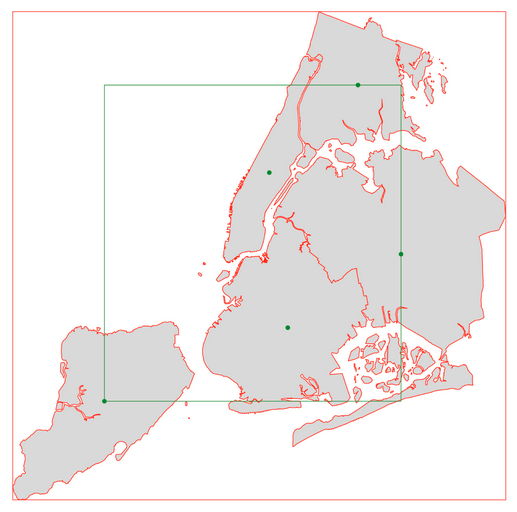
\includegraphics[width=6cm]{bounding-box.png}
                \end{figure} 

            \end{itemize}
        \end{itemize}
        \item Dissolving features
        \begin{itemize}
            \item \textit{sf::st\_union()} 
            \begin{itemize}
                \item Dissolves polygons into a single polygon
                \item Clusters individual points into a MULTIPOINT geometry
            \end{itemize}
        \end{itemize}
        \item Convex Hull
        \begin{itemize}
            \item Used to create tighter bounding box around points
            \begin{itemize}
                \item Need to cluster individual points (e.g. centroids) into MULTIPOINTS before drawing convex hull
            \end{itemize}
            
            \begin{figure}[h]
                \centering
                \caption{Convex hull example}
                \label{convex hull}
                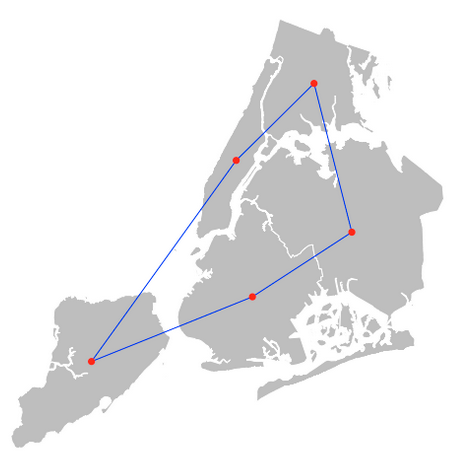
\includegraphics[width=6cm]{convex-hull.png}
            \end{figure} 
            
            \item Can be created around buffers that overlap
            
            \begin{lstlisting}[language=R]
                # Buffer the beech trees by 3000
                beech_buffer <- st_buffer(beech, dist = 3000)

                # Limit the object to just geometry
                beech_buffers <- st_geometry(beech_buffer)

                # Dissolve the buffers
                beech_buf_union <- st_union(beech_buffers)

                # Plot the dissolved buffers
                plot(beech_buf_union)

                # Create the convex hull
                beech_hull <- st_convex_hull(beech_buf_union)
            \end{lstlisting}

            \begin{figure}[h]
                \centering
                \caption{Overlapping buffers that can be used in a convex hull}
                \label{convex hull buffer}
                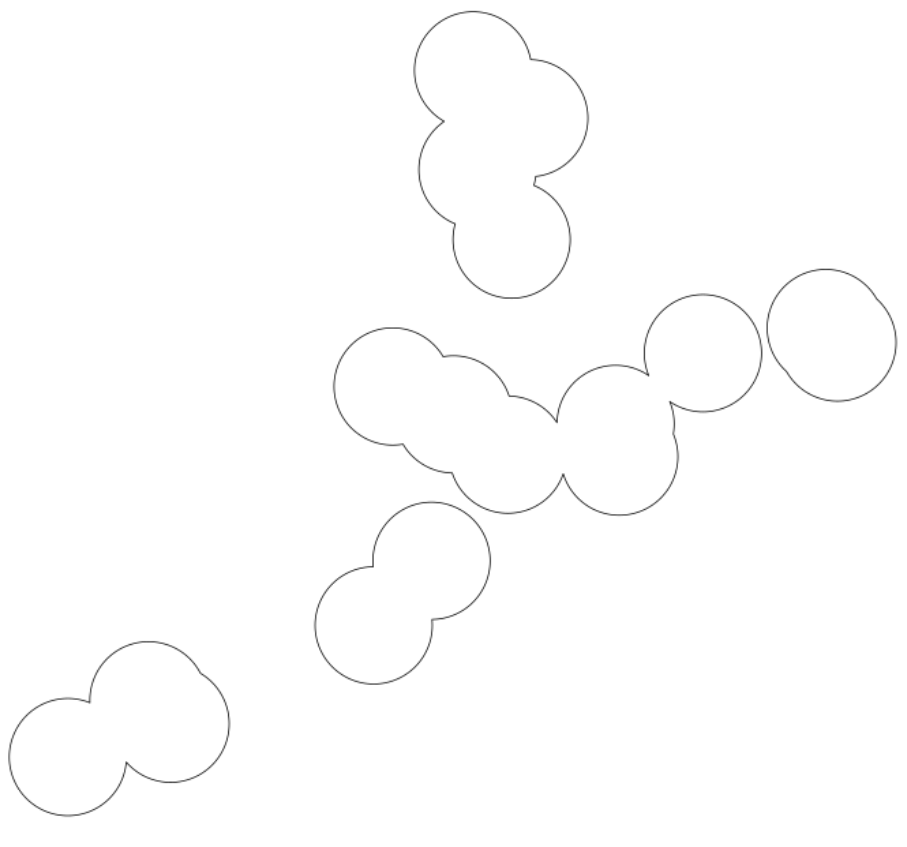
\includegraphics[width=6cm]{convex-hull-buffer.png}
            \end{figure} 

        \end{itemize}
    \end{itemize}
    \item Multilayer geoprocessing and relationships
    \begin{itemize}
        \item \textit{sf::st\_join(out\_df, attr\_df)} used to join two dataframes with spatial information when there are not columns that can be used to link them, so need to join based on geographic information
        \begin{itemize}
            \item First object is the df you want as the output (contains most useful information)
            \item Second object is the df that contains the attributes you want added
        \end{itemize}
        \item \textit{sf::st\_intersects(large\_df, small\_df)} shows which geographies intersects
        \begin{itemize}
            \item \textit{sf::st\_intersection(large\_df, small\_df)} clips the resulting list so only those that intersect are shown, and not the rest of the polygons
        \end{itemize}
        \item \textit{sf::st\_contains(large\_df, small\_df)} shows which geographies are completely contained in another polygon
        \item \textit{sf::st\_distance(feat1, feat2)} calculates distances between features
    \end{itemize}
    \item Geoprocessing with rasters
    \begin{itemize}
        \item \textit{raster::mask(raster, mask = poly)} to mask all areas but the polygons of interest
        \item \textit{raster::crop(raster, mask = poly)} to crop the raster to just include the polygons (cf. bounding box) 
        \item\textit{raster::extract(raster, poly, fun = mean)} extracts the values from polygons as a list using a function (e.g. NULL returns all values, and mean returns the means from each polygon)
        \item \textit{raster::overlay(raster1, raster2, fun = func)} allows you to perform functions to rasters e.g. first raster contains elevation, second contains the multiplication values, and the function says to multiple the two rasters together
    \end{itemize}
    \item \textit{ggplot2::geom\_sf()} can create maps of \textit{sf} data
    \begin{itemize}
        \item \textit{aes(fill = var)} used to create choropleths
    \end{itemize}
    \item \textit{tmap::tmap\_arrange(map1, map2, nrow)} allows you to plot multiple maps in a grid
\end{itemize}

\section{Datacamp: Spatial statistics in R}

\begin{itemize}
    \item The `window' is the study area where events (e.g. points) occur
    \item Spatial point pattern is the set of observed events and the window
    \item Spatial point process is stochastic process that generates the points in a window
    \item Most of spatial point pattern analysis is trying to infer the spatial point process that would produce the dataset (pattern)
    \item The `mark' are the values observed e.g. height of tree etc
    \item \textit{spatstat} package very useful
    \begin{itemize}
        \item Stores spatial point patterns in \textit{ppp} objects (planar point pattern)
    \end{itemize}
    \item Quadrat test used to test spatial randomness
    \begin{itemize}
        \item Split window into even subregions
        \item Count number of events in each subregions 
        \item Plot histogram of event counts vs number of quadrants
        \item Should follow Poisson distribution if random
        \item Use Chi-squared test for observed vs expected
        \item \textit{spatstat::quadrat.test()}
    \end{itemize}
    \item Generally, points can be generated in two different manners:
    \begin{enumerate}
        \item Regular (inhibitory) processes that are completely random and follow a uniform Poisson distribution
        \begin{itemize}
            \item \textit{spatstat::rpoispp()} useful for generating Poisson point process i.e. spatially random points
        \end{itemize}
        \item Clustered processes where points occur more together than under a uniform Poisson process
        \begin{itemize}
            \item Thomas process is a clustered pattern where `parent' points are uniformly distributed and `child' points are clustered around the parent
            \begin{itemize}
                \item \textit{spatstat::rThomas()} useful for generating a Thomas process
            \end{itemize}
            \item Strauss process is a clustered pattern with a \textit{repulsive} point pattern i.e. no points can be closer than a threshold
            \begin{itemize}
                \item \textit{spatstat::rStrauss()}
                \item Sometimes called regularly spaced
            \end{itemize}
        \end{itemize}
    \end{enumerate}
    \item Quadrat test can lose power with too few or too many subregions
    \item Other tests don't rely on arbitrary subregions and rely on estimated properties of the process
    \begin{itemize}
        \item Nearest neighbour distributions
        \begin{itemize}
            \item Plot histogram of NN distances
            \item Plot cumulative distribution of NN distances (\textit{G(r)}) (\textit{spatstat::nndist()})
            \item Poisson distribution can be used to calculate cumulative distribution curve ($G(r) = 1 - exp( - \lambda \pi r^2)$)
            \item \textit{spatstat::Gest()} estimates function \textit{G(r)}
            \item Need to use edge-correction as events near the edge of the window have less area for a nearest neighbour
        \end{itemize}
        \item Ripley's reduced second moment measure (K function)
        \begin{itemize}
            \item K is the number of expected events to occur within a given distance scaled by the intensity
            \item Calculate for all points and plot events vs distance (\textit{spatstat::Kest()})
            \item For completely random event, should be $\pi \times d^2$
            \item Needs edge corrections, like \textit{G(r)} test
            \item Use Monte-Carlo test
            \begin{itemize}
                \item Simulate spatially random point patterns in your window and calculate K function plots, before overlaying observed K function
                \item Calculate \textit{envelope} (the minimum and maximum values at each distance) \textit{spatstat::envelope(ppp, Kest, correction)}
                \item If larger than simulations at any point - indication of clustering at distance
                \item If smaller than simulations - indication of inhibitory process
                \item If use 99 simulations can calculate p-value easily (1/(99+1)) (assuming it is the largest value)
                \item $plot(K\_cluster\_env, . - pi * r^2 \sim r)$ used to subtract expected K function of Poisson process to help visualize
            \end{itemize}
        \end{itemize}
    \end{itemize}
    \item Bivariate point pattern
    \begin{itemize}
        \item Point pattern map with colors representing different outcomes e.g. cholera vs not cholera
    \end{itemize}
    \item Cross nearest neighbour function
    \begin{itemize}
        \item Similar to NN but measure nearest distances between \textbf{case and control} events
    \end{itemize}
    \item Cross K-function
    \begin{itemize}
        \item Similar to K-function, but number of control events expected within radius of case events
    \end{itemize}
    \item Null hypothesis for cross-functions is that the proportion of each type is uniform over space
    \begin{itemize}
        \item Simplest test is that the cross-functions are identical to regular \textit{G(r)} and \textit{K(r)} functions for cases/controls i.e. no location where cases occur more often that expected
        \item Can estimate and map rate of cases over study area
        \begin{enumerate}
            \item Work out intensity of cases over area
            \item Work out intensity of cases and controls over area
            \item Divide 1) by 2) to get proportion of cases
            \item Use kernel smoothing to get continuous estimate of intensity
            \begin{enumerate}
                \item Replace each point in the point pattern with a `kernel'
                \begin{itemize}
                    \item Simple localized 2D function centered on the point
                \end{itemize}
                \item Add up all the kernels to get smooth intensity
            \end{enumerate}
            \begin{itemize}
                \item \textit{spatstat::density()} will produce kernel density estimates
                \item \textit{spatstat::split()} will split categorical data into separate point patterns that can be used to calculate and visualize relative proportions (density ratios)
                \item \textit{spatialkernel::spseg(, opt = 3)} will calculate bandwith for kernel function (use CV to optimize kernel smoothing)
                \begin{itemize}
                    \item Use to compute ratio and spatial estimate of the rate of cases
                    \item \textit{opt = 3} indicates want to calculate p-values
                \end{itemize}
            \end{itemize}
            \item Use Monte-Carlo simulation to calculate uncertainty in estimate
            \begin{enumerate}
                \item If there are 200 cases out of 1000 total events, produce 99 simulations where the 200 cases are randomly selected from any of the 1000 events using the kernel function to weigh likelihoods
                \item Compare density ratio from data to simulated density ratios
                \item Can plot density ratio estimates with significant areas highlighted based on comparison to simulated densities
                \begin{itemize}
                    \item \textit{spatialkernel::plotmc()}
                \end{itemize}
            \end{enumerate}
        \end{enumerate}
    \end{itemize}
    \item Space-time
    \begin{itemize}
        \item Time point process also has window, but instead has min and max time points, not a polygon
        \item Usually both spatial and temporal clustering
        \item Sometimes clusters in both dimensions
        \begin{itemize}
            \item Spatial and temporal processes not independent
        \end{itemize} 
        \item Can use space-time K function
        \begin{itemize}
            \item Expected number of points within distance \textit{d} and time \textit{t}
            \begin{itemize}
                \item Creates cylindrical volume of space-time
            \end{itemize}
            \item If spatial and temporal processes independent
            \begin{itemize}
                \item $K_{st}(s, t) = K_s(s) \times K_t(t)$
                \item Test independence by checking how two sides of equation differ
                \item $D(s, t) = K_{st}(s, t) - K_s(s) \times K_t(t)$
                \item $D(s, t) \approx 0$
            \end{itemize}
            \item Test significance using Monte-Carlo simulation for permutation test
            \begin{itemize}
                \item Randomly permute event times
                \item Retains spatial distribution, just breaks links between space and time
                
                \begin{figure}[h]
                    \centering
                    \caption{Space-Time Monte-Carlo simulation method}
                    \label{space time mc}
                    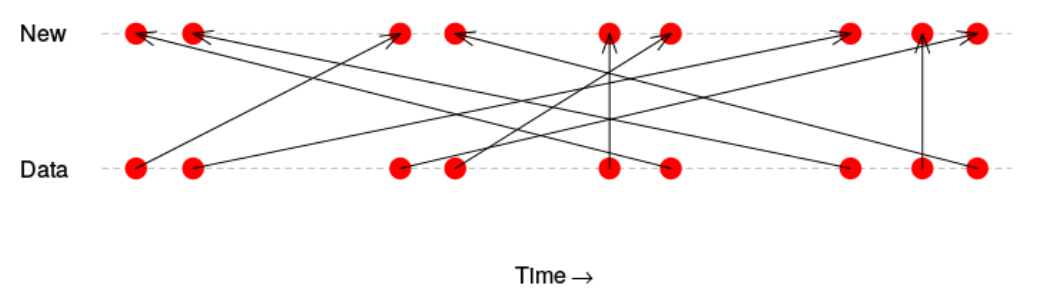
\includegraphics[width=10cm]{space-time-mc.png}
                \end{figure}

                \item  Compare observed $D(s, t)$ vs distribution of simulated values
            \end{itemize}
            \item \textit{splancs::stmctest()} used, but requires matrix rather than df
        \end{itemize}
    \end{itemize}
    \item Often don't have point data, e.g. due to confidentiality, instead have areas with subregions summarized
    \begin{itemize}
        \item \textit{spdep::spplot(spdf, "var")} good way to quickly create choropleth
    \end{itemize}
    \item Simple null hypothesis is that regions are spatially random
    \begin{itemize}
        \item Alternative is that there is local spatial structure i.e. neighbours might be more similar than expected under random hypothesis
        \begin{itemize}
            \item \textbf{Spatial autocorrelation}
        \end{itemize}
        \item Define neighbours:
        \begin{itemize}
            \item Adjacent: 2 regions that share a boundary
            \item Any two regions within a distance
            \item \textit{spdep::poly2nb()} calculates the neighbours of polygons and creates an \textit{nb} object
        \end{itemize}
        \item Moran I statistic tests local similarity
        \begin{equation}
            I = \frac{n}{\sum_i \sum_j w_{ij}} \frac{\sum_i \sum_j w_{ij} (z_i - \bar{z})(z_j - \bar{z})}{\sum_i (z_i - \bar{z})^2}
        \end{equation}
        \begin{itemize}
            \item Sum of contributions from two neighbouring pairs
            \item If two neighbours both above or below mean, then positive amount
            \begin{itemize}
                \item Neighbours are similar
            \end{itemize}
            \item If two neighbours either side of mean, then contributes a negative amount
            \begin{itemize}
                \item Neighbours are dissimilar
            \end{itemize}
            \item Use MC simulation by randomly arranging numbers over region and compare observed I statistic to distribution of I statistics
            \item \textit{spdep::moran.test(var, wnb)}
            \begin{itemize}
                \item Needs a weighted \textit{nb} object
                \item \textit{spdep::nb2listw()} creates weighted \textit{nb} object
            \end{itemize}
        \end{itemize}
    \end{itemize}
    \item Use \textit{Standardized Mortality Ratio} to observe difference in health data between regions
    \begin{itemize}
        \item $SMR_i = \frac{O_i}{E_i}$
        \item Create \textit{Exceedance Probability Map}
        \begin{itemize}
            \item Triggers alert when SMR in region is above threshold with certain probability (using binomial distribution to calculate CIs and distribution around SMR)

\begin{lstlisting}[language=R]
    # Probability of a binomial exceeding a multiple (e) of expected deaths
    binom.exceed <- function(observed, population, expected, e){
        1 - pbinom(e * expected, population, prob = observed / population)
    }
\end{lstlisting}

        \end{itemize}
    \end{itemize}
    \item Generalized Linear Models can be fit to spatial data
    \begin{itemize}
        \item $Y \sim N(X \beta, \sigma^2)$ standard linear model formula
        \item $Y \sim D(\mu(X \beta))$ equation for generalized linear models
        \begin{itemize}
            \item $D$ is the distribution chosen
            \item $\mu$ is the \textit{link function} that transforms the $X \beta$ term appropriately for the distribution
            \item e.g. $Y \sim \text{Poisson}(\exp(X \beta))$ where $D =$ Poisson, and $\mu = \exp()$ 
        \end{itemize}
        \item Should visualize residuals vs map to check if there is spatially smooth correlation
        
        \begin{figure}[h]
            \centering
            \caption{Map residuals to check for spatially smooth correlation}
            \label{spatial residuals}
            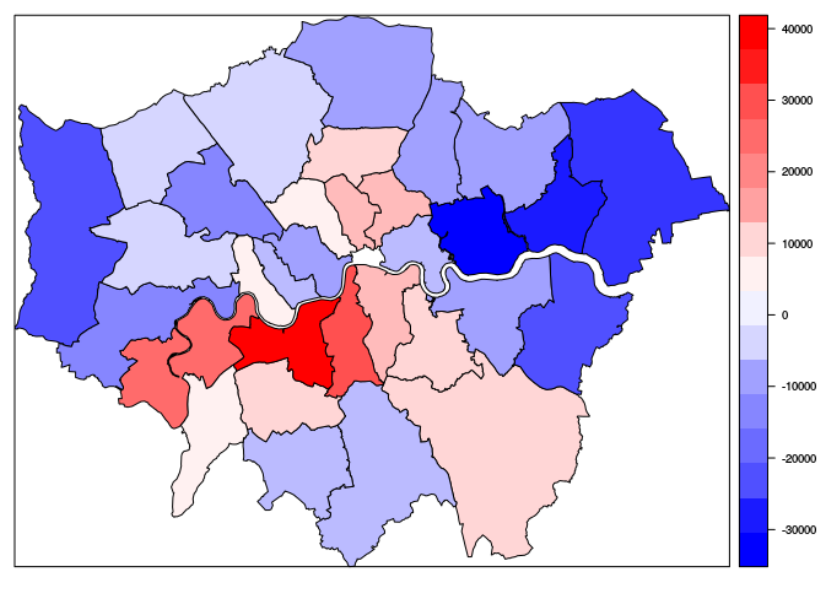
\includegraphics[width=7cm]{spatial-residuals.png}
        \end{figure}

        \item \textit{spdep::moran.mc(res, wnb)} can use Monte-Carlo simulation to test if spatial correlation of residuals using a weight \textit{nb} object
        \item Dealing with spatially correlated residuals
        \begin{enumerate}
            \item See if variable not included in model can be used to explain correlation e.g. age-structure of population, or pollution intensity, by refitting model with added variables
            \item Add spatial feature to model to create a \textbf{conditional auto-regression (CAR)} model
            \begin{itemize}
                \item $Y = X \beta + S(x, y)$
                \item $S(x, y)$ could be a continuous function over space, but can be easier to define for each unit
                \begin{itemize}
                    \item $S_i \sim N(\bar{S}_{j \sim i}, \sigma_i^2)$ is one example where for a region $i$, $S$ comes from normal distribution with  mean equal to mean of the neighbouring regions, with variance to be fitted
                    
                    \begin{figure}[h]
                        \centering
                        \caption{BYM spatial correlation linear model component}
                        \label{bym spatial correlation}
                        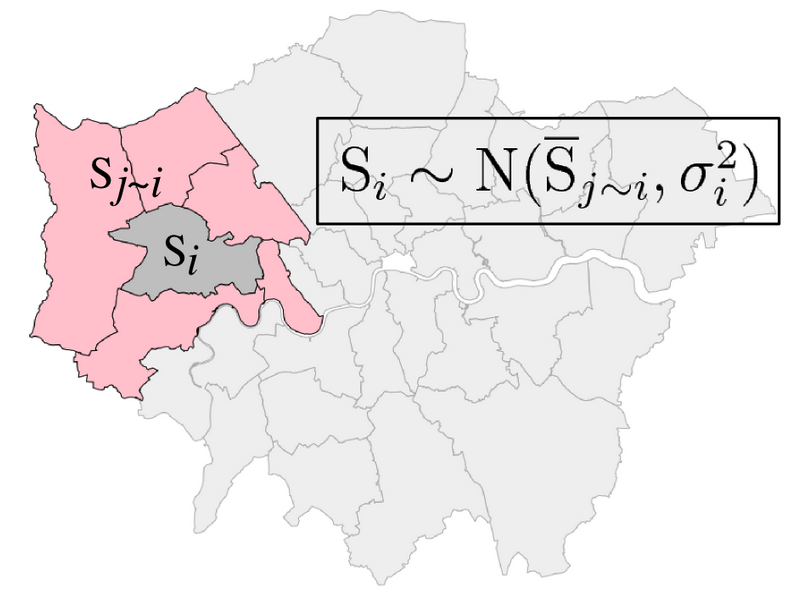
\includegraphics[width=8cm]{bym-spatial-correlation.png}
                    \end{figure}

                \end{itemize}
                \item Hard to maximise likelihood, so instead used Bayesian inference
                \begin{itemize}
                    \item Don't get mean and variance of normal distribution of parameter
                    \item Instead get samples that give posterior distribution of parameter - the probability distribution of a parameter given the data
                    \item Use samples to compute credible intervals of posterior distribution
                    \item \textit{R2BayesX::bayesx(resp ~ vars + sx(i, bs = "spatial", map = gra))} used to add spatial component
                    \item \textit{gra} object required for map (not \textit{nb}) so use \textit{R2BayesX::nb2gra(nb)} to convert
                    \item \textit{residuals(mod\_fit)[, "mu"]} will add residuals to \textit{spdf} based on rates, not counts, so can be compared across regions with different populations
                \end{itemize}
            \end{itemize}
        \end{enumerate}
    \end{itemize}
    \item Measurement type will vary geostatistical method used e.g. continuous vs count
    \item Initial geostatistical approaches
    \begin{enumerate}
        \item Map variables to see large-scale trend
        \begin{itemize}
            \item Fit trends explicitly as function of coordinates
        \end{itemize}
        \item Show strips in one direction (anisotropy - directionality)
        \begin{itemize}
            \item Consider anisotropic effects
        \end{itemize}
        \item Discontinuities where values change rapidly
        \begin{itemize}
            \item Model need to add barriers when calculating distance
        \end{itemize}
    \end{enumerate}
    \item Need to describe correlations between points by distance
    \begin{itemize}
        \item Variogram cloud
        \begin{itemize}
            \item Plots half the squared difference between points vs distances
            \begin{itemize}
                \item Known as the \textbf{semi-variance}
                \item Half because difference between A-B is the same as B-A
            \end{itemize}

            \begin{figure}[h]
                \centering
                \caption{Variogram cloud}
                \label{variogram cloud}
                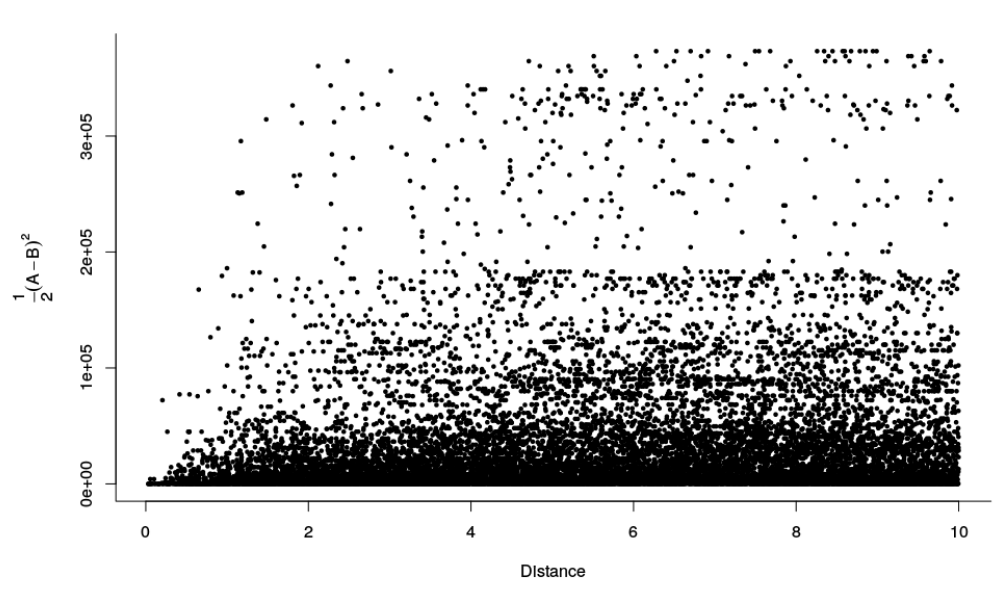
\includegraphics[width=14cm]{variogram-cloud.png}
            \end{figure}

            \item \textit{gstat::variogram(resp $\sim$ coords, cloud = TRUE)}
        \end{itemize}
        \item Variogram (incorrectly also called ``semi-variogram'')
        \begin{itemize}
            \item Bin the variogram cloud distance
            \item Average the values in each bin
            \begin{itemize}
                \item Enough values to provide a good estimate of the mean
            \end{itemize}
            \item Plot mean values vs center of the distance bins
            \item If semivariance flattens off, semivariance = variance of the data
            \item Fit model to variogram
            \begin{itemize}
                \item Current preferred model is the \textbf{matern} class of model due to its differentiability properties
            
                \begin{equation}
                    C(d) = \sigma^2 \frac{2^{(1 - \nu)}}{\Gamma (\nu)}\left(\sqrt{2 \nu}\frac{d}{\rho}\right)^\nu K_\nu \left(\sqrt{2 \nu}\frac{d}{\rho}\right)
                \end{equation}
                
                \item \textit{gstat::fit.variogram(vario, model = vgm(parms))}
                \item Have to estimate parameters (nugget, partial sill, range)
            \end{itemize}
        \end{itemize}
    \end{itemize}
    \item Kriging uses model fit from variogram and interpolates data points
    \begin{itemize}
        \item Simplest when response is continuous variable that is assumed to be Guassian (normally distributed)
        \item Prediction variance smallest when closest to data points
        \begin{itemize}
            \item If nugget = 0, then estimate will go through the data point
        \end{itemize}
        \item \textit{gstat::krige(form, val\_df, miss\_df, model = vario)} will predict the missing values
    \end{itemize}
    \item Prediction maps
    \begin{itemize}
        \item Will use kriging, but first need to create a \textit{SpatialPixels} object
        
\begin{lstlisting}[language=R]
    # ca_geo, geo_bounds have been pre-defined
    ls.str()

    # Plot the polygon and points
    plot(geo_bounds); points(ca_geo)

    # Find the corners of the boundary
    bbox(geo_bounds)

    # Define a 2.5km square grid over the polygon extent. The first parameter is
    # the bottom left corner, the second is the width and height of each 
    # rectangle in the grid. The third specifies the number of rectangles in
    # each direction.
    grid <- GridTopology(c(537853, 5536290), c(2500, 2500), c(72, 48))

    # Create points with the same coordinate system as the boundary
    gridpoints <- SpatialPoints(grid, proj4string = CRS(projection(geo_bounds)))
    plot(gridpoints)

    # Crop out the points outside the boundary
    cropped_gridpoints <- crop(gridpoints, geo_bounds)
    plot(cropped_gridpoints)

    # Convert to SpatialPixels (sp object equivalent)
    spgrid <- SpatialPixels(cropped_gridpoints)
    coordnames(spgrid) <- c("x", "y")
    plot(spgrid)
\end{lstlisting}

        \item Pass \textit{SpatialPixels} grid as the new data to the \textit{gstat::krige()} function
        \item \textit{automap::autoKrige(form, input\_data, new\_data, model)} will quickly fit variogram and use kriging
        \begin{itemize}
            \item Pass to \textit{plot()} function to plot kriging predictions, standard error, and variogram
            \item Use a \textit{SpatialPixels} grid to produce a surface rather than individual points
            \item Need to carefully check results to make sure the results make sense e.g. has small nugget and rises to reach sill
            \item Only possible when meets assumption of Guassian data
        \end{itemize}
    \end{itemize}
    \item Working with non-Guassian data in kriging
    \begin{itemize}
        \item Trans-Guassian kriging transforms sample values to approximate Guassian distribution
        \item Model-based geostatistics
        \begin{itemize}
            \item Use bayesian statistics for inference e.g. Markov-Chain Monte-Carlo samplers to estimate paramter distributions
            \item Computationally intensive
        \end{itemize}
        \item Nested variograms
        \begin{itemize}
            \item Spatial correlation may not be well-fit to single variogram function
            \begin{itemize}
                \item Particularly if spatial structure on more than one level
            \end{itemize}
            \item Fit variograms to different components and create combined function
            \item May be possible to overfit and precise fit may not affect final model output much
        \end{itemize}
    \end{itemize}
\end{itemize}

\section{Datacamp: Interactive maps with leaflet with R}

\begin{itemize}
    \item Leaflet uses `tiles' to create layers of maps e.g. basemap, markers etc
    \begin{itemize}
        \item Specify different tile using \textit{leaflet::addProviderTiles()}
    \end{itemize}
    \item Use \textit{ggmap::geocode(location = "address")} to return lon-lat for address
    \item Set default view using two different methods
    
    \begin{figure}[h]
        \centering
        \caption{Set Leaflet default view}
        \label{leaflet default view}
        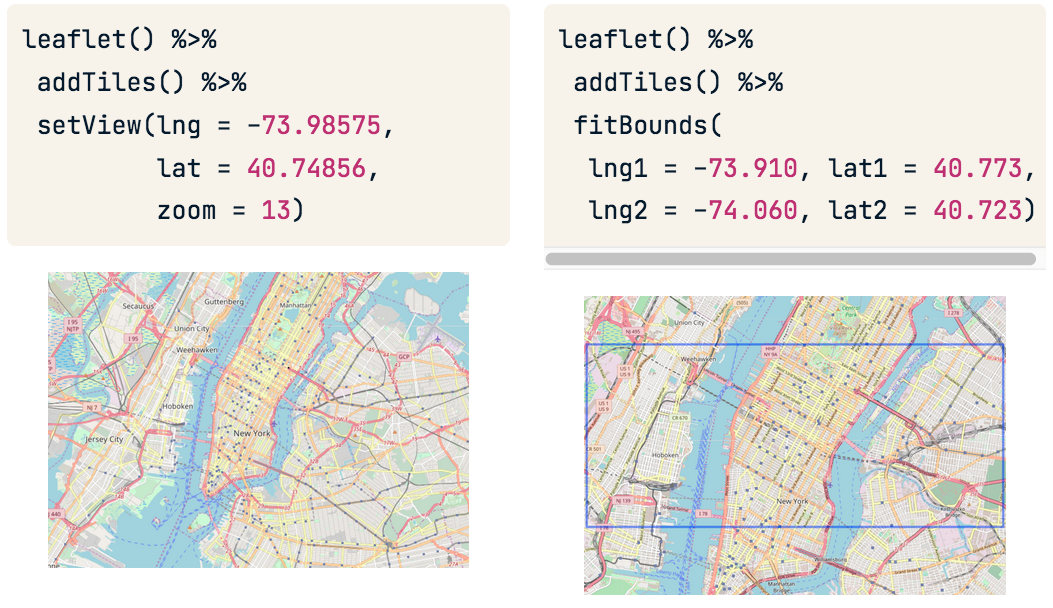
\includegraphics[width=14cm]{leaflet-default-view.png}
    \end{figure}
    
    \begin{itemize}
        \item \textit{leaflet::clearBounds()} removes previously saved default views
    \end{itemize}
    \item Can restrict panning etc using \textit{leaflet::leaflet(options = leaflet\_options(minZoom = x, dragging = FALSE))}
    \item \textit{leaflet::addMarkers(lng = df\$lon, lat = df\$lat, popup = df\$desc)} can add markers from a df with text descriptions that show when clicked
    \begin{itemize}
        \item \textit{leaflet::addPopups()} alternative that don't show markers
        \item \textit{leaflet::clearMarkers()} removes previously added markers
        \begin{itemize}
            \item Useful if saved basemap object and want to replace markers for specific map
            \item \textit{leaflet::addCircleMarkers()} can be a useful alternative when pin markers overlap - similar to scatter plot
        \end{itemize}
    \end{itemize}
    \item If you pipe the data to the map, no need to specify dataframe for every option e.g. longitudes etc.
    \begin{itemize}
        \item Need to use the $\sim$ symbol though e.g. \textit{leaflet::addCircleMarkers(label = $\sim$paste0(``\textless b \textgreater'', name, ``\textless /b \textgreater''))}
        \begin{itemize}
            \item Specifying \textit{label} instead of \textit{popup} means the information is available on hover, rather than click
        \end{itemize}
    \end{itemize}
    \item To add color to markers, polygons etc:
    \begin{enumerate}
        \item Specify a colour palette (depends on variable type) e.g.:
        \begin{itemize}
            \item \textit{pal \textless- colorFactor(palette = c(``red'', ``blue'', ``\#9b4a11''), levels = c(``Public'', ``Private'', ``For-Profit''))}
            \item \textit{pal \textless- colorNumeric(palette = ``reds'', domain = c(1:50), reverse = TRUE)}
            \item \textit{pal \textless- colorBin(palette = ``reds'', bins, domain = c(1:50))}
            \item \textit{pal \textless- colorQuantile(palette = ``reds'', n, domain = c(1:50))}
        \end{itemize}
        \item \textit{leaflet::addCircleMarkers(col = $\sim$pal(var))}
        \item Add legend
        \begin{itemize}
            \item \textit{leaflet::addLegend(pal = pal, values = c(``Public'', ``Private'', ``For-Profit''), opacity, title, position)}
        \end{itemize}
    \end{enumerate}
    \item Can make map more easily searchable with \textit{leaflet.extras} package
    \begin{itemize}
        \item Can geocode directly in the map without needing \textit{ggmap::geocode()}
        \item \textit{addSearchOSM()} allows users to search for locations
        \item \textit{addReverseSearchOSM()} shows lon and lat when picked dropped
        \item \textit{addResetMapButton()} provides an icon to revert to default view
        \item \textit{addSearchFeatures(targetGroups, options = searchFeaturesOptions(zoom))} allows users to search specific groups of markers and zoom in once identified
    \end{itemize}
    \item Can add markers in layers to allow groups to be toggled on and off
    \begin{itemize}
        \item Have to create subsets of the dataframe before adding separately
        \begin{itemize}
            \item Because adding in layers, order matters to stacking
        \end{itemize}

\begin{lstlisting}[language=R]
    # Load the htmltools package to clean up characters that may be 
    # interpreted as HTML
    library(htmltools)

    # Create data frame called public with only public colleges
    public <- filter(ipeds, sector_label == ``Public'')  

    # Create a leaflet map of public colleges called m3 
    m3 <- leaflet() %>% 
            addProviderTiles(``CartoDB'') %>% 
            addCircleMarkers(
                data = public, radius = 2, label = ~htmlEscape(name),
                color = ~pal(sector_label), group = ``Public''
                ) %>%
            addLayersControl(overlayGroups = c(``Public''))
\end{lstlisting}

    \end{itemize}
    \item Similarly, can add multiple basemap layers
    \begin{itemize}
        \item Only one can be viewed at a time
        
\begin{lstlisting}[language=R]
    leaflet() %>% 
        addTiles(group = ``OSM'') %>%
        addProviderTiles(``CartoDB'', group = ``Carto'') %>% 
        addProviderTiles(``Esri'') %>% 
        addLayersControl(baseGroups = c(``OSM'', ``Carto'', ``Esri''))
\end{lstlisting}

        \item Last basemap layer will be the one that is shown, unless chosen otherwise using toggle

    \end{itemize}
    \item Can cluster observations together
    \begin{itemize}
        \item \textit{addCircleMarkers(clusterOptions = markerClusterOptions())}
    \end{itemize}
    \item Can create choropleths
    \begin{itemize}
        \item \textit{leaflet::addPolygons(weight, color, label, highlight = highlightOptions)}
        \item \textit{pal \textless- colorBin(palette = ``reds'', bins, domain = sp@data\$var)}
    \end{itemize}
    \item \textit{htmlwidgets::saveWidget()}
\end{itemize}



\end{document}